\documentclass{amia}
\usepackage{graphicx}
\usepackage{listings}
\usepackage[labelfont=bf]{caption}
\usepackage[superscript,nomove]{cite}
\usepackage{color}
\usepackage{caption}


\newcommand\YAMLcolonstyle{\color{red}\mdseries}
\newcommand\YAMLkeystyle{\color{black}\bfseries}
\newcommand\YAMLvaluestyle{\color{blue}\mdseries}

\makeatletter

% here is a macro expanding to the name of the language
% (handy if you decide to change it further down the road)
\newcommand\language@yaml{yaml}

\expandafter\expandafter\expandafter\lstdefinelanguage
\expandafter{\language@yaml}
{
  keywords={true,false,null,y,n},
  keywordstyle=\color{darkgray}\bfseries,
  basicstyle=\YAMLkeystyle,                                 % assuming a key comes first
  sensitive=false,
  comment=[l]{\#},
  morecomment=[s]{/*}{*/},
  commentstyle=\color{blue}\ttfamily,
  stringstyle=\YAMLvaluestyle\ttfamily,
  moredelim=[l][\color{orange}]{\&},
  moredelim=[l][\color{magenta}]{*},
  moredelim=**[il][\YAMLcolonstyle{:}\YAMLvaluestyle]{:},   % switch to value style at :
  morestring=[b]',
  morestring=[b]",
  literate =    {---}{{\ProcessThreeDashes}}3
                {>}{{\textcolor{red}\textgreater}}1     
                {|}{{\textcolor{red}\textbar}}1 
                {\ -\ }{{\mdseries\ -\ }}3,
}

% switch to key style at EOL
\lst@AddToHook{EveryLine}{\ifx\lst@language\language@yaml\YAMLkeystyle\fi}
\makeatother

\newcommand\ProcessThreeDashes{\llap{\color{cyan}\mdseries-{-}-}}
\begin{document}


\title{i2b2 implemented over SMART-on-FHIR} 
\author{Nicolas Paris, Degrees$^{1}$, Firstname B. Lastname, Degrees$^{2}$}

\institutes{
    $^1$Institution, City, State, Country (if applicable); $^2$Institution, City, State, Country (if applicable)\\
}

\maketitle

\noindent{\bf Abstract}

\textit{Integrating Biology and the Bedside (i2b2) is the de-facto open-source medical tool for cohort discovery. Fast Healthcare Interoperability Resources (FHIR) is a new standard for exchanging health care information electronically. Substitutable Modular third-party Applications (SMART) defines the SMART-on-FHIR specification on how application shall interface with EHR thought FHIR. In this paper, we extended i2b2 for being plugged on top of one or multiple SMART-on-FHIR API. This enable federation queries, security, terminology mapping, and also bridges the gap between i2b2 and modern big-data technologies.}
%[h150  words]Programmatic themes: Translational
%Keywords: Cohort Discovery, Data integration and standardization, Informatics implementation

\section*{Introduction}
% A short background and objective(s) of the study

%\textit{FHIR} is becoming a standard for application to share EHR data and defines multiple resources representing multiple concepts (clinical, organisation\ldots). FHIR defines specification to. FHIR rapid success is partly du to the adoption of robust and widely used technologies such REST, json that made the success of internet major.
%
%\textit{SMART} success improve the user experience exaclty the same major internet provide access to many application with a single authentification.
%
%\textit{i2b2} is the de-facto open-source medical tool for cohort discovery and allows phisician to easily have translational view of their patients. Many initiatives have extended this primary goal with statistical analysis on place[ref], federating queries over multiple centers [shrine, insite, triknetX], and even genomics analytics.[transmart, i2b2-transmart]. It's recent migration on github makes possible multiple developpers to improve and extend the source code. I2b2 has been described to be used by more than 200 hospital over the world.
%The tool is flexible and can support its own stars schema and ontology model, or exploit OMOP common data model[]. Monthly ETL processes are generaly feeding the databases has time, resource, maintenance and disk space consuming processes. The database layer can be PostgreSQL, Oracle or Microsoft SQL Server. While those transfers in those relational databases are still feaseable these days, the emmergence of connected object and big-data generation let the methodology in the future incertain.
%
%This work is a general interface between i2b2 \& FHIR, exploiting the FHIR search[ref], Terminology Mapping[ref] and  SMART Oauth2 security[ref] specifications. The results does not only bridge the gap between two active communities, it opens to i2b2 new areas for data federation, data type hangling, security, interoperability and addresses the problem described above.

Learning Health Systems aim to maximize the potential of large-scale, harmonized data from variable, quickly-developing digital sources including Electronic Health Records (EHRs) emerging as a powerful tool to facilitate discoveries that can improve health.. Data heterogeneity is one of the critical problems in analyzing, reusing, sharing or linking datasets. With the development of platforms enabling the linking and federation of phenome, genome and exposome data across sites  in US(1�4, Europe (5,6 or at international scale (7 a key challenge is to define harmonized access to heterogeneous EHR-based data.

In the domain of patient care, several large-scale efforts have been underway for over a decade with the goal of specifying both the structure and the semantics of patient clinical information in a manner that enables computable semantic interoperability between diverse systems. Two major contributions to the interoperability of clinical information currently dominate internationally: i) the ISO EN 13606 is a generic and comprehensive representation for the interchange of EHR information between heterogeneous systems suited to the extraction, communication and/or mapping of longitudinal EHR data or of fine grained parts of an EHR. The openEHR Foundation maintains a more detailed model, catering for the widest set of use cases for patient level data; ii) the Health Level Seven (HL7) Fast Healthcare Interoperability Resources (FHIR), built on lessons from previous standards including the Reference Information Model (RIM) that became an ISO standard in 2003 and Clinical Document Architecture, designed to express a single clinical document as a message using HL7 version 3 RIM classes.

Both EN ISO 13606 and HL7 FHIR standards define the semantics of patient care data and clearly demonstrate the need for �layers of semantic expressiveness� including: i) generic reference information models of concepts and relationships (e.g. EN ISO 13606, openEHR Reference Model or FHIR model) each capable of binding terms from terminology models (e.g. SNOMED-CT, LOINC, etc.) and associated with a data type models such as ISO 21090; and ii) more detailed models (e.g. EN ISO 13606 or openEHR Archetypes/Templates or FHIR resources). 

Although there is no consensus in the medical informatics community regarding a standard patient information model, HL7 FHIR specifications are gaining interest and show promise to mitigate the classic site-specific data mapping problem. FHIR specifies a RESTful application programming interface (API) to access resources. Several initiatives ima ti facilitate the adoption of FHIR, including the Argonaut project (8, the Data Access Framework (9 and the Clinical Information Modeling Initiative (CIMI) launched in 2011, an international consortium of representing national bodies, Standards Development Organizations, healthcare organizations and vendors are building collaboratively a process and tools for constructing a single curated collection of shared implementable clinical information models that are free for use at no cost (10.

SMART Health IT is an open, standards based technology platform that enables innovators to create apps that seamlessly and securely run across the healthcare system. Using an electronic health record (EHR) system or data warehouse that supports the SMART standard, patients, doctors, and healthcare practitioners can draw on this library of apps to improve clinical care, research, and public health (11. SMART success improve the user experience exaclty the same major internet provide access to many application with a single authentification.

i2b2 is the de-facto open-source medical tool for cohort discovery and allows  healthcare practitioners to easily query patient data to address research questions. Many initiatives have extended this primary goal with statistical analysis on place[ref], federating queries over multiple centers [shrine, insite, triknetX], and even genomics analytics.[transmart, i2b2-transmart]. Its recent migration on github allows multiple developers to improve and extend the source code. I2b2 has been described to be used by more than 200 hospitals over the world. The tool is flexible and can support its own stars schema and ontology model, or exploit new information models � e.g. PCORnet  or OMOP common data model - without requiring changes to the underlying data .ETL processes feeding the databases are time, resource, maintenance and disk space consuming processes. The database layer can be PostgreSQL, Oracle or Microsoft SQL Server. Though ETL processes are still feasible these days, the emergence of high throughput healthcare data data and the Internet of Things requires the development of new approaches.

This work describes a general interface between i2b2 and any type of EHRexploiting the FHIR search[ref], Terminology Mapping[ref] and SMART Oauth2 security[ref] specifications. The aim was not only to bridge the gap between patient care and research communities, but also toopen to i2b2 new areas for  better data type , security and interoperability management in the context of scalable solutions for cross border and cross domain networking of data.
\section*{Methods}
% Design, setting (if appropriate), patients or participants (if appropriate), interventions (if appropriate), and main outcome measurement

The Figure \ref{fig1} shows the overall architecture and how the 3 tier i2b2 application articulates with 3 remote instution. The figure shows how i2b2 application gives access to users in a SMART-on-FHIR application context. In this context, users log one time in any SMART application or EHR, and get acces to their specialized applications available. Moreover, the architecture allows to mix queries over multiples endpoints: zero to one i2b2 star schema and/or zero to many SMART-on-FHIR APIs.

The Figure \ref{fig2} is a detailled UML. The scenario describes a user who query over an i2b2 instance with multiple remote FHIR-endpoints accesses. 
The user first logs-in with its personnal secrets informations, that are verified by the i2b2 project management cell (i2b2pm). The i2b2pm then asks and stores a Oauth2 credential to all the SMART authentication services with it's own i2b2 connection details (one global secret for the i2b2 application) dedicated for the user. The i2b2pm returns then an i2b2 project list, to let the user choose and access according its habilitation details defined into i2b2. The user builds and run a multiple panel query accross different medical domains to get back a patient cohort set. The i2b2crc will then loop the following steps over each panel and each SMART-on-FHIR API. The i2b2crc transforms the query according to the FHIR-search specifications  and passes it with the credentials to the FHIR-API. The Oauth2 credential information are verified by the FHIR-API, and the query extended with the coding with synonyms defined in the terminology conceptMapping. The resulting query is then translated by the FHIR-API in the local database dialect to fetch the result. The result is transformed into a FHIR json bundle only containing the information needed (patient\_ids in this case). A parsing step extract the patient\_ids. They are mapped to an i2b2 unique identifier thanks to the existing i2b2 patient\_mapping features, to be then pushed into a CRC temporary table that integrates all the results. Once looping done, the i2b2crc applies the patients security steps to the CRC tmp table in order to only keep the patients that are available for the project selected by the user. The patient cohort set is finally returned to the user.

\begin{figure}[h!]
\centering
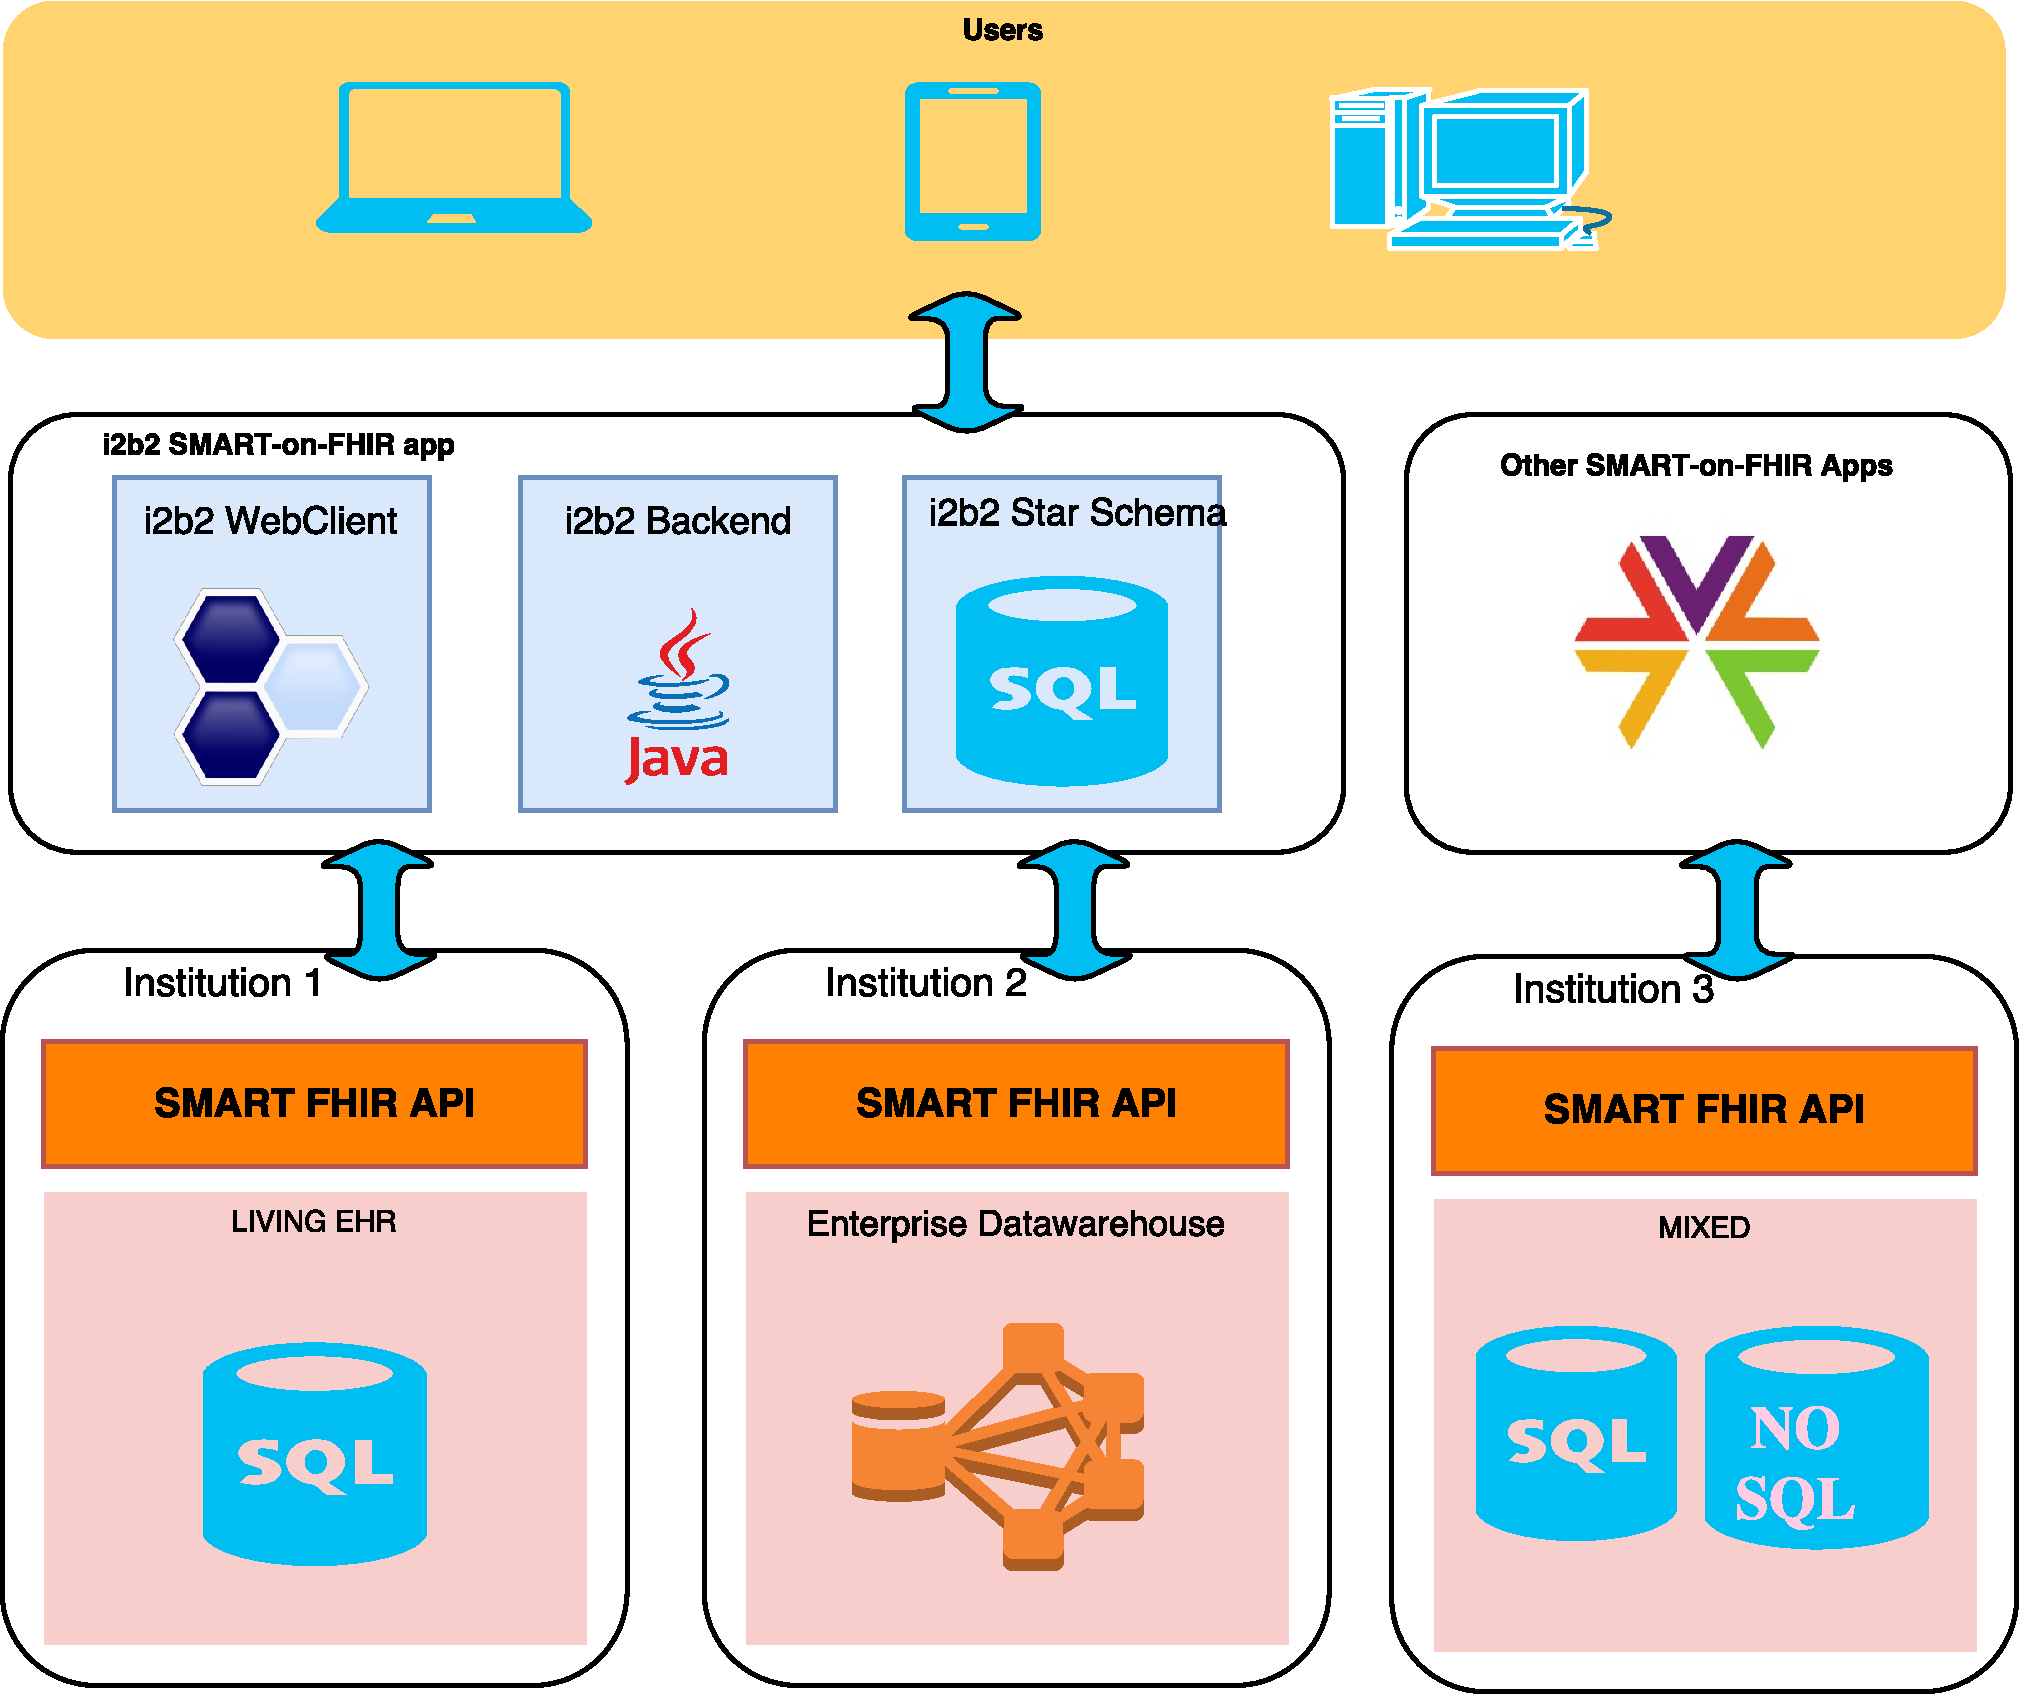
\includegraphics[scale=.4]{overall.pdf}
	\caption{Overall Diagram}
\label{fig1}
\end{figure}

\begin{figure}[h!]
\centering
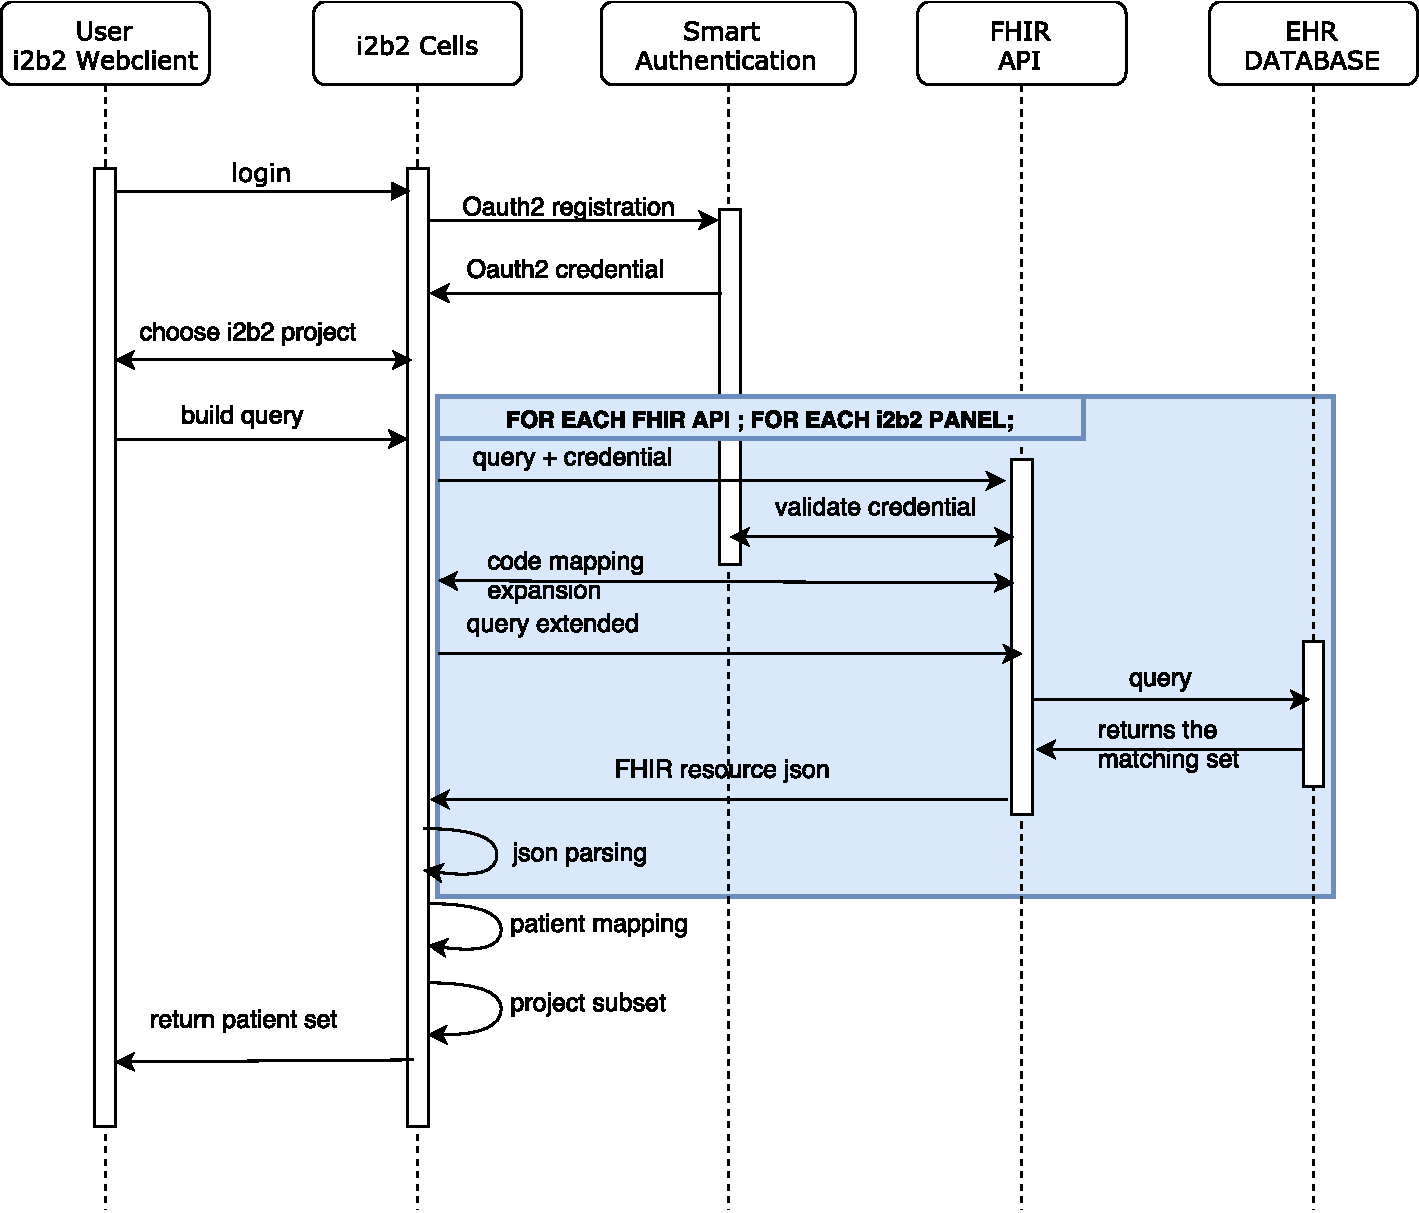
\includegraphics[scale=.5]{diagram_sequence.pdf}
\caption{UML Sequence Diagram}
\label{fig1}
\end{figure}
%- sequence diagram (user, i2b2, i2b2 database, smart, EMR database)
%- Example of http queries produced by i2b2-fhir-search
%- Optimisation, ask only for elements needed by i2b2


\textit{Outcome measurement:}In order to test the FHIR DSTU3 68 resources coverage compatibility, the HAPI FHIR test server has been used has endpoint since it contains useful demo datasets. The benchmark comparing traditionnal i2b2 and FHIR-i2b2 has been done with the same i2b2 observation\_fact table (postgresql 9.6). The first is based on a 1.7 i2b2 incance. The FHIR-i2b2 has been setup by implementing HAPI-FHIR server on top of the observation\_fact table into an apache tomcat 9 webserver, and accessed via a the FHIR-i2b2 prototype. The FHIR-i2b2 big-data benchmark has been setup by implementing HAPI-FHIR server on top of a MIMICiii table multiplied by 15, and stored in a apache HIVE2 table distributed over a 5 computer cluster in ORC format.

\section*{Results}
% Key findings

\begin{figure}[h!]
\centering
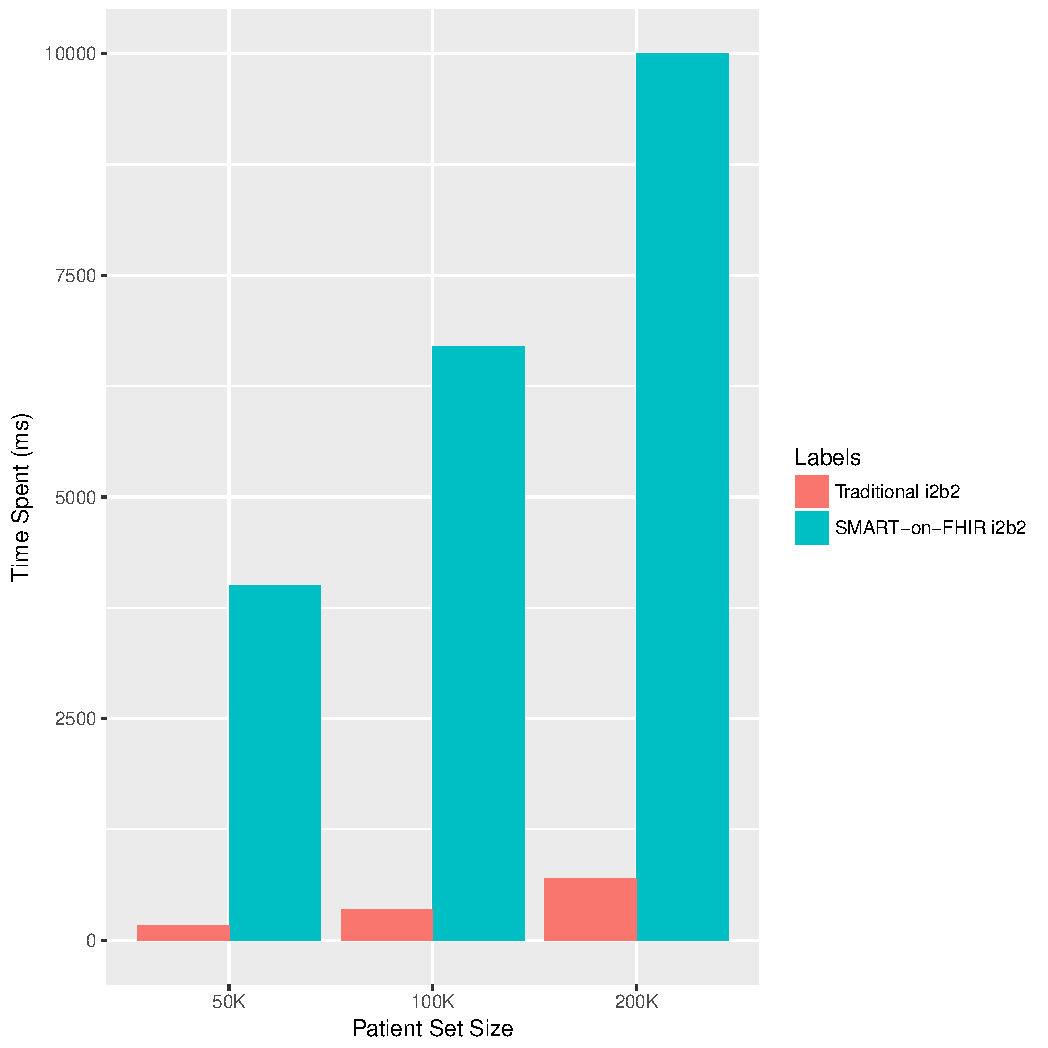
\includegraphics[scale=.7]{graph2.pdf}
	\caption{Traditionnal versus SMART-on-FHIR performances comparison (on a 150M postgreSQL table)}
\label{fig1}
\end{figure}

\begin{figure}[h!]
\centering
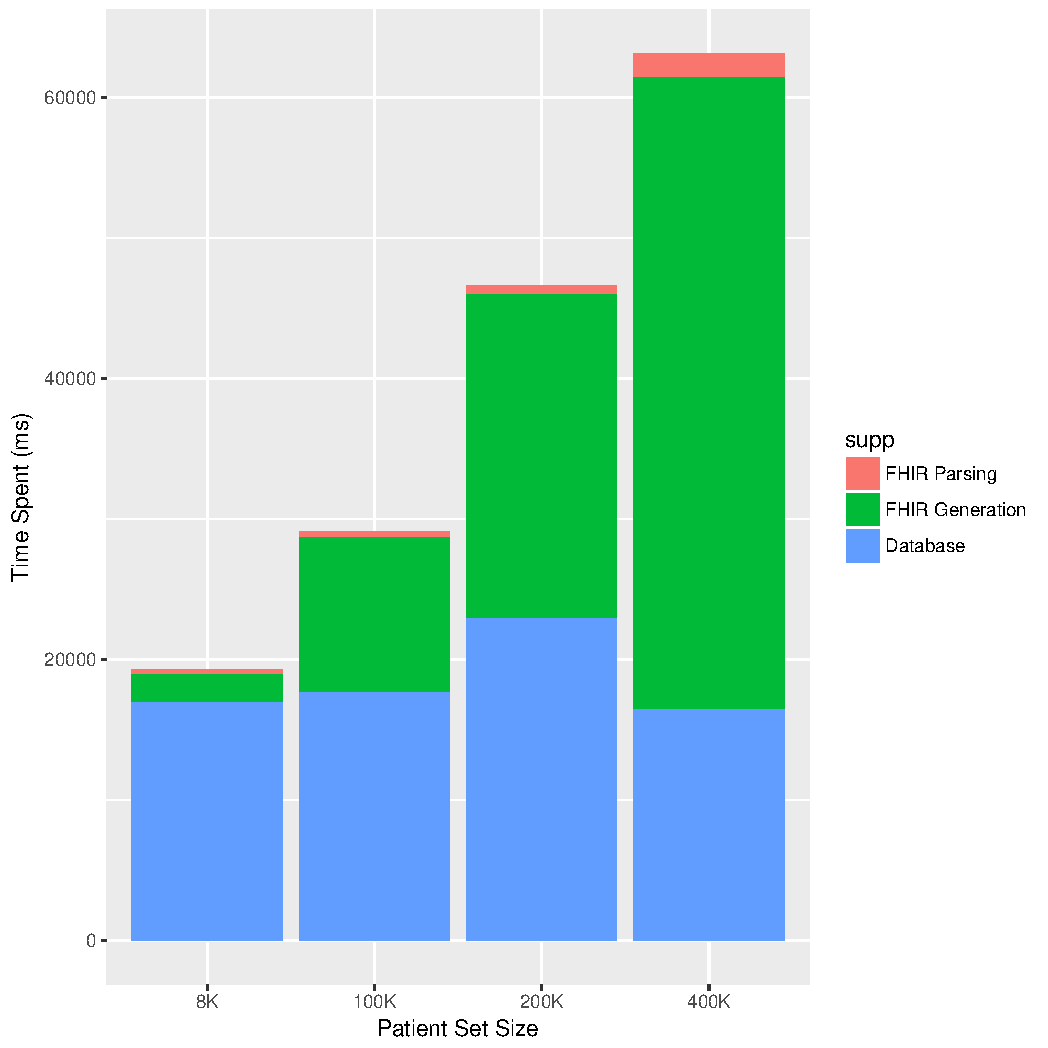
\includegraphics[scale=.7]{graph1.pdf}
	\caption{SMART-on-FHIR performances (on a 5B Hive table)}
\label{fig2}
\end{figure}
\begin{figure}[h!]
\centering
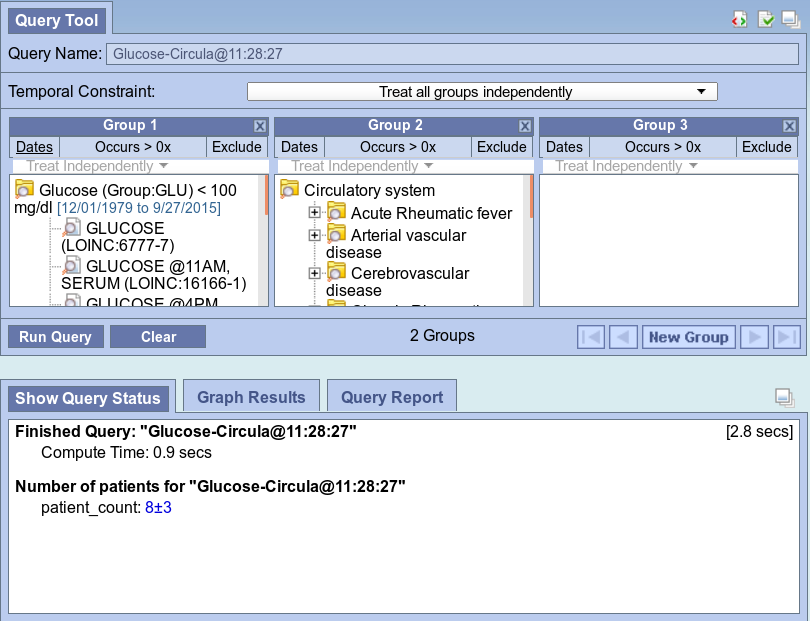
\includegraphics[scale=.5]{demo.png}
	\caption{SMART-on-FHIR online demo screenshot}
\label{fig3}
\end{figure}
\textit{Implementation Status: } The design presented below is not yet fully implemented. To date, the query builder is able to query on both star schema and one remote FHIR endpoint at a time. Logical relation between selection criteria represented as multiple i2b2 webclient panels are also possible. The constitution of a patient\_set is working and allows to apply constraint by dates, by values and by one or multiple codes. The code expansion based on FHIR terminology mapping is also implemented. A living demo is deployed at http://34.205.31.28/webclient/ and provided the screenshot presented in Figure \ref{fig3}. The panel 1 query searched into HAPI FHIR test server for patients with a set of loinc glucose codes having value lower than 100ml/dl in a range of 1979 to 2015 and mixed with the panel 2 with i2b2 patients having diagnosed related to circulatory system. The resulting patient\_set is about 8 patients.

\textit{Performances: } The performances have been benchmarked (Figure \ref{fig1})versus a traditionnal i2b2 instance based on star schema with the same amount of data, and configuration. The histogram shows traditionnal are 20 times faster than the FHIR based version. The difference can be explained by the additionnal steps involved: the fetched resultset is transformed into a json bundle, sent over the network and then parsed. The performance factor tends to decrease with number of patient fetched. The second benchmark (Figure \ref{fig2}) experienced connecting to a apahce HIVE table on a HDFS big-data platform. The results shows the performances are compatible under the minute. Moreover, the barplot shows the major bottleneck is the FHIR Generation step. Such amount of data have never been described to be handle by i2b2 before since we approach here traditionnal RDBMS limitations. While traditionnal i2b2 outperforms the FHIR based one on modest datasets, the latter opens new perspectives by allowing to connect to specialized and optimized database systems.

\begin{figure}
\begin{lstlisting}[language=yaml]
---
version: dstu3
Patient:
    patientUriPath: $.resource.id
    patientUriField: id
Observation:
  - patientUriPath: $.resource.subject.reference,
  - encounterUriPath: $.resource.context.reference
  - instanceUriPath: $.resource.id
  - datePath: $.resource.effectiveDateTime
  - patientUriField: subject
  - encounterUriField: context
  - instanceUriField: id
  - dateField: effective
[...]
---
\end{lstlisting}
  \caption{FHIR resource YAML configuration file}
	\label{conf1}
\end{figure}

\textit{i2b2 feature coverage: }i2b2 querying feature covers filtering patients facts by code, values, dates, thought patient history, within an encounter temporal window or even a free sequence of events. By adding new temporal table mechanisms, the present work allows all those features. Ence, it does not limit the existing set of functionalities. The Table \ref{tab1} shows how those feature are covered. The i2b2-FHIR configuration file Figure \ref{conf1} describes contains jsonPATH, which json elements contain respectively the patient ID, encounter ID, fact ID, and dates values. This is how i2b2 deliberation mecanisms can be populated, and the set build.

\textit{Security: }A security layer has been proposed and implemented into the existing CRC cell. A new i2b2 table allows to define witch patient are part of wich project. This security layer is important because it allows with one endpoint with all patients records, to create multiple projects with subset. In terms of performances, the table might be vertivally partitionned and splitted by project, in order to get stable performances while number of project will increase. This mecanism is both compatible with traditionnal i2b2 and i2b2-SMART-on-FHIR and has been deployed in production and handle more than distinct 200 projects.
The Oauth2 security layer has not yet been implemented. The implementation will inspire from project\cite{ref2,ref3} that recently succeed in.

\textit{Extensibility:} The FHIR access layer has been tested over the HAPI FHIR test server for all resources at least to refearing to a patient (68 resources), and does have a complete resource coverage. To date, the query builder is conpatible with last FHIR DSTU3 version. In the future, it will be compatible with each FHIR release, and maintain backward compatibilities. The FHIR version of each endpoint is setup in the configuration file (Figure \ref{conf1}). The query builder handles the FHIR extensibility, local profiled resources or even local new resources. Moreover, the design allows to filter based on FHIR extensions (https://www.hl7.org/fhir/extensibility.html\#extension). The results let conclude the design is flexible enougth to query multiple centers with different fHIR implementation at the same time.

\textit{Interoperability: }FHIR conceptMapping objects have been produced to make the proof of concept. The Table \ref{tab2} shows the HTTP query used to retrieve the equivalent code. The concpetMapping are then parsed to only collect the "exact-matches" codes. The FHIR-search query is then extended with the collected code-systems/codes. The design allows to query multiple FHIR endpoints using diffetent terminologies. However, this does not allow to match valuesets. While their is some field of improvement, the results open area for massive and collaborative concept mapping, with a terminolgy server ready.
By querying over the conceptMapping resources, the CRC cell is able to expand the query to fetch all synonyms. This design allows implementers to align accross different code systems, or to define mapping within the same code system. Since the FHIR-configuration allows to use a specific ConceptMapping endpoint, this allows to federate queries and use only one terminology server where concept mapping is done in collaboration.

\begin{table}[h!]
\centering
	\begin{tabular}{|p{2cm}|p{6cm}|p{5cm}|}
  \hline
		\textbf{ontology table columns}    & \textbf{Description} & \textbf{Example} \\ \hline
		c\_basecode  &  FHIR code\_system / code pipe separated  & FHIR:http://loinc.com$|$1234-5  \\ \hline
		c\_facttable  &  Resource / Profile pipe separated  & Observation$|$ObservationAphp  \\ \hline
		c\_metadataxml  &  An xml describing datatype (numeric, free text or enumerated) and measure units  & cf: i2b2 documentation   \\ \hline
		c\_concept\_cd  &  an optionnal additional filter  & active=true\&status=final  \\ \hline
  \end{tabular}
	\label{tab1}
\caption{i2b2 ontology adapted for FHIR}
\end{table}

\begin{table}[h!]
\centering
	\begin{tabular}{|p{6cm}|p{10cm}|}
  \hline
    \textbf{HTTP request}    & \textbf{Description}  \\ \hline
		GET $<$FHIR-BASE$>$/$<$Resource$>$\newline?\_elements=$<$elements$>$\&code=$<$codes$>$\newline\&date=gt$<$date\_inf$>$\&date=lt$<$date\_sup$>$\newline\&$<$custom\_filter$>$  & Retrieves choosen $<$elements$>$ from resources optionally matching a date range or/and a list of $<$codes$>$  or/and a $<$custom\_filter$>$     \\ \hline
	 GET $<$FHIR-BASE$>$/ConceptMapping\newline?target-code=$<$codes$>$\&target-system:in=$<$code-system$>$  & Retrieves all codes that are mapped to $<$codes$>$ \& $<$code-system$>$   \\ \hline
  \end{tabular}
	\label{tab2}
\caption{Index of HTTP requests}
\end{table}


\section*{Conclusion} 

The main contribution of the work is to pave the way for cohort-generation process by leveraging standard access, with interoperable terminology systems and state of the art security methods. The hospital centers international effort to converge to FHIR data exchange layer[ref] will ease the data-federation to query center without dedicated datawareouhsing staff.

The secondary contribution of the work is to allow implementers to use their technology, and will allow i2b2 instance to benefits from the fast past and future improvements on big-data technologies.

All together, this works opens a new-area of specific solution to apprehend the medical diversity, variety and volumetry.

\section*{Discussion}
% Key conclusions with direct reference to the foundational or methodological advancement or biomedical application
%- the performances open new area such Genomics\cite{ref4}, Imaging, Physiological Monitoring or even for i2b2 applications to discover new cohorts.
%- the security is renforced and allows multiple sub project to acces to subset of the whole patients. This addresses the patient research opposition and allows studies to only access to data they need. Moreover, it brings the last security technologies and allows federated architechture possible.
%- free text search: FHIR search specification covers filtering by dates, values or eaven basic operation on strings. However, it is not intended to allow text retrieval to mine the free-text notes. The abstraction provided by the FHIR layer allows to plug new text specific technologies based on apache lucene, such SOLR \& Elastic search. This will allow clinitian to mine text as simple as modern search engine does.
%- the interoperability gain from FHIR interface let envisage to query multiple center the same way on real-time data. This design allows two opposite paradigm. The first each clinitian is able to query i2b2 with it's own local terminologies he uses to code with. The second is to choose a Common Terminology Model as a pivotal, and map all the local coding to it. In both cases, the concept mapping remain to be done in many institution. Since all are based on different languages, different granularity and different concept and practices, this remains a challenge to be adressed.

By introducing into i2b2 a dependency on FHIR specifications, this will lead to bring together community and improve both sides.

Several modules have been implemented, some aspects of the design have only been tested as separate modules.
The roadmap provides for the development of multiple SMART-on-FHIR endpoints access, Oauth2 implementation and performances improvements. Once satisfied with the results, the system should be available in next releases of core i2b2. Specific exploration around specialized databases (temporal-series, text-mining, distributed, graph databases) will result to better handling variety of big-data, such genomic[ref], textual notes, DICOM imaging, physiological waveforms or exposomic.

While all resource containing patient reference where tested, there is a need to propose a general mapping between traditional i2b2 objects (patient, visit, provider, observation) and FHIR specific resources (Organization, HealthcareService, Patient, EpisodeOfCare, Condition, Procedure, Medication, MedicationRequest, Observation, DiagnosticReport, ClinicalImpression\ldots)
A general algoritme to translate FHIR terminologies into i2b2 ontology will also be investigated, and result as a complementary sofware.

Last but not least concept mapping between many institutions and languages remains to be done. Since all are based on different languages, different granularity and different concept and practices, this remains a challenge to be adressed. While ontology matching has a long exp, this research area is still challenging.

%\section*{Conclusion}
%Your conclusion goes at the end, followed by References, which must follow the Vancouver Style (see: www.icmje.org/index.html).  References begin below with a header that is centered.  Only the first word of an article title is capitalized in the References. 
%\section*{Another Major Heading and References}
%This sentence has two reference citations\cite{ref1,ref2}.
%
%More text of an additional paragraph, with a figure reference (Figure ~\ref{fig1}) and a figure inside a Word text box below.  Figures need to be placed as close to the corresponding text as possible and not extend beyond one page.\\
%\begin{figure}[h!]
%\centering
%\includegraphics[scale=1]{pics/figure1.png}
%\caption{Total allergy alerts, overridden alerts, or drug order cancelled.}
%\label{fig1}
%\end{figure}
%
%This is additional text added just to show the one-column formatting.  This is additional text added just to show the one-column formatting.  This is additional text added just to show the one-column formatting.  This is additional text added just to show the one-column formatting.  This is additional text added just to show the one-column formatting.  This is additional text added just to show the one-column formatting.  This is additional text added just to show the one-column formatting.
%
%This paragraph contains a reference to a table just below (Table 1).  All tables need to be placed as close to the corresponding text as possible, But each individual table should be on one page and not extend to multiple pages unless labeled as ``��Continued"��.
%
%\begin{table}[h!]
%\centering
%\caption{Submission type, abstract length, and page length maximum for AMIA submissions.}
%  \begin{tabular}{|l|l|l|}
%  \hline
%    \textbf{Submission Type}    & \textbf{Abstract Length}  & \textbf{Page Length Maximum**} \\ \hline
%    Paper  & 125-150 words  & Ten   \\ \hline
%    Student Paper  & 125-150 words  & Ten \\ \hline
%    Poster  &50-75 words*   & One \\ \hline
%    Podium  Abstract & 50-75 words*  & Two \\ \hline
%    Panel   &150-200 words  & Three \\ \hline
%    System Demonstrations    &150-200 words  & One \\ \hline
%  \end{tabular}
%	\label{tab1}
%\end{table}
%*: All podium abstract and poster submissions must have a brief (50-75 words) abstract. The abstract does NOT have to be part of the document, but must be entered on the submission website in the Abstract box in Step 2.
%
%**: \textcolor{red}{If your submission is longer than what is specified below, it will be rejected without review.}
%
%This is another paragraph.


\makeatletter
\renewcommand{\@biblabel}[1]{\hfill #1.}
\makeatother



\bibliographystyle{unsrt}
\begin{thebibliography}{1}
\setlength\itemsep{-0.1em}

\bibitem{ref1}
Pryor TA, Gardner RM, Clayton RD, Warner HR. The HELP system. J Med Sys. 1983;7:87-101.
\bibitem{ref2}
Gardner RM, Golubjatnikov OK, Laub RM, Jacobson JT, Evans RS. Computer-critiqued blood ordering using the HELP system. Comput Biomed Res 1990;23:514-28.

\bibitem{ref2}
Wagholikar KB, Mandel JC, Klann JG, Wattanasin N, Mendis M, Chute CG, et al. SMART-on-FHIR implemented over i2b2. Journal of the American Medical Informatics Association. 2016 Jun 6;ocw079. 

\bibitem{ref3}
Pfiffner PB, Pinyol I, Natter MD, Mandl KD. C3-PRO: Connecting ResearchKit to the Health System Using i2b2 and FHIR. Seo J-S, editor. PLOS ONE. 2016 Mar 31;11(3):e0152722. 

\bibitem{ref4}
Alterovitz G, Warner J, Zhang P, Chen Y, Ullman-Cullere M, Kreda D, et al. SMART on FHIR Genomics: Facilitating standardized clinico-genomic apps. Journal of the American Medical Informatics Association. 2015 Jul 21;ocv045. 

\end{thebibliography}
\end{document}
